\documentclass[a4paper, 12pt]{report}

\usepackage{pdfpages}
\usepackage[ra={Livrable 1 - P2I2}, subjectAcronym=PPII2]{configfrancaisCM}

\title{Rapport}
\author{DIONISIO, FREY, BILLARD, MEZUREUX}
\date{\today}

\begin{document}

\maketitle
\dominitoc
\mtcsettitle{minitoc}{}
\tableofcontents

\chapter{Introduction}
\minitoc
\chaptermark{Introduction}
\clearpage
    
    \section{Contexte et objectifs du projet}

Ce projet s'inscrit dans le cadre pédagogique de notre première année d'étude en école d'ingénieur au sein de l'établissement Telecom Nancy. L'objectif y est de mettre en pratique les compétences scientifiques et techniques acquises tout au long de cette première année en se rapprochant d'une étude de cas concrète.
\bigskip

Il se divise en deux étapes distinctes. Il nous a été demandé dans un premier temps de construire en langage "C" un programme qui permet de planifier un parcours de charge pour un véhicule électrique et pour un trajet donnés et d'enrichir cette application en y incorporant les ajouts de notre choix. Dans un second temps, il nous a fallut réaliser toujours en langage "C" un module de simulation qui pour un ensemble d'usagers, calcule le taux de charge des bornes du territoire.
\bigskip

Notons également que tout au long du projet nous avons dû suivre une gestion de projets rigoureuse, ce
qui nous a permis d’assurer une planification efficace et un suivi approprié des activités. Nous étions
obligé d'adopter une approche méthodologique solide, afin d’assurer que notre projet soit réalisé de manière efficace, dans les délais impartis.
\bigskip

Toute l’équipe a pris plaisir à travailler sur le projet et nous tenons à remercier tous ceux qui nous
ont aidés.

    \section{Objectifs du rapport}

Ce rapport synthétise le travail réalisé par l'équipe de PoinCarWash pour répondre à la problématique posée. À savoir travailler à l'élaboration d'outils utiles au développement d'une mobilités plus écologique.
    
\bigskip
Le présent rapport fait état de la conception et de l'implémentation de notre travail mais également des performances et des tests sur ce dernier ainsi que d'une présentation de notre gestion de projet.

    \section{Présentation du plan}

Au cours de ce rapport, nous aborderons dans un premier temps les éléments de gestion de projet communs aux deux étapes. Cette première partie nous permettra ainsi de justifier nos choix d'approches méthodologiques pour la réalisation de ce projet.
\bigskip

Nous procéderons ensuite de manière similaire pour les deux étapes du projet. En premier lieu, nous décrirons les éléments de gestion de projet spécifiques à chacune d'elles. Nous détaillerons ensuite les phases de conception et de développement avant d'enfin présenter les performances et les tests de nos applications.
\bigskip


Pour conclure nous récapitulerons les résultats obtenus dans chaque partie du projet en les mettant en parallèle avec les objectifs fixés au départ, nous analyserons les avantages et les limites de notre travail, et formulerons des recommandations pour de futures améliorations et développements avant de conclure définitivement le projet.


\chapter{Gestion de projet}
\minitoc
\chaptermark{Gestion de projet}
\clearpage
    \section{Définition du projet}
        
    \subsection{Contexte et justification du projet}

Avec la prise de conscience écologique grandissante dans la population, les citoyens et les Etats se tournent progressivement vers des modes de consommation et des politiques plus responsables et écologiques. La Commission européenne a dans cette optique récemment pris la décision d'interdire la vente de véhicules thermiques à l'horizon 2035. Le développement et l'utilisation des véhicules électriques va donc connaître une croissance élevée dans les années à venir. En effet, selon les premières projections\footnotemark[1], le marché des véhicules électirifiés pourrait représenter 24\% des parts de marché d'ici 2025 et 90\% d'ici 2040. 
\bigskip
\footnotetext[1]{Selon l'étude \href{https://about.bnef.com/electric-vehicle-outlook/}{BloombergNEF}}

Pourtant, voyager dans ce type de véhicules peut encore parfois s'avérer difficile, notamment en ce qui concerne leur autonomie encore relativement limitée et la répartition des bornes de recharge sur le territoire, cette dernière étant encore très inégale sur le sol français. Il est donc nécessaire pour faciliter leur adoption d'en faciliter et d'en optimiser l'utilisation.
\bigskip

La première étape de notre projet consiste alors en la conception d'un algorithme permettant de calculer pour un utilisateur le trajet le plus court entre un point A et un point B situés en France, en optimisant ses passages aux bornes de recharges. Cet outil pourra aider les conducteurs à naviguer plus efficacement et à ainsi surmonter les inquiétudes liées à l'autonomie limitée des voitures électriques.
\bigskip

La seconde étape du projet est elle basé sur l'étude du remplissage des stations en fonction d'une base de trajets données. L'acquisition de ces statistiques pourrait par exemple permettre de planifier plus efficacement l'expansion future du réseau de recharge.
\bigskip

Ainsi nous espérons au travers de ce projet promouvoir une mobilité plus durable en participant à l'élaboration de solutions pratiques pour surmonter les obstacles liés à l'autonomie et à la disponibilité de stations de recharge pour véhicules électriques.
\bigskip

        \subsection{Portée du projet}

\textbf{\underline{Objectifs du projet} :}
\begin{itemize}
  \item Conception d'un algorithme de calcul d'itinéraire optimisé pour véhicule électrique
  \item Conception d'une application de monitoring du remplissage des stations de recharge
\end{itemize}
\bigskip

\textbf{\underline{Ressources} :}
\begin{itemize}
  \item Groupe de projet (4 personnes) : temps de travail variable pendant 9 semaines
  \item Equipe pédagogique de Telecom Nancy : aide ponctuelle
  \item Bases de données relatives aus stations de recharge et aux véhicules électriques
\end{itemize}
\clearpage

\textbf{\underline{Livrables} :}
\begin{itemize}
  \item Code source des deux applications, \textbf{24 Mai}
  \item Guide utilisateur décrivant l'installation du programme et les modalités de son utilisation, \textbf{24 Mai}
  \item Rapport du projet incluant les éléments relatifs à la gestion de projet et décrivant les choix motivés des structures de données et des algorithmes (sur la base d'un état de l'art détaillé), les
fonctions réalisées et leur analyse (complexité mémoire, temps), les fonctions réalisées et les tests mis en œuvre, \textbf{24 Mai}
\end{itemize}
\bigskip

\textbf{\underline{Éléments non prévus dans le projet} :}
\begin{itemize}
  \item Adaptation du calcul des itinéraires en fonction du taux de remplissage des stations de recharges.
\end{itemize}

        \subsection{Parties prenantes}

\textbf{\underline{Identification} :}
\begin{itemize}
  \item Interne :
  \begin{itemize}
      \item Groupe de projet : Les participants directs au projet, responsables de la conception et du développement des outils demandés.
  \end{itemize}
  \item Externe :
  \begin{itemize}
      \item Enseignants et jury : Ils guident et évaluent les étudiants dans le cadre du projet.
      \item Autres groupes : D'autres groupes de projet travaillant sur des sujets similaires, avec lesquels des échanges et des discussions peuvent être initié pour partager des idées et des connaissances.
  \end{itemize}
\end{itemize}
\bigskip

\textbf{\underline{Evaluation de l'influence et de l'importance} :}
\begin{itemize}
    \item Groupe de projet : Influence élevée et importance élevée, car ils sont directement responsables de la réalisation du projet et de l'atteinte des objectifs fixés.
    \item Enseignants/jury : Influence élevée et importance élevée, car ils évalueront le projet et fourniront des conseils et des orientations pour assurer la qualité et la réussite du projet.
    \item Autres groupes de projet : Influence faible à moyenne et importance faible à moyenne, car ils peuvent partager des connaissances et des expériences similaires, mais leur impact direct sur le projet est limité.
\end{itemize}
\bigskip

On peut synthétiser cette analyse au traver de ce diagramme:

\begin{center}
    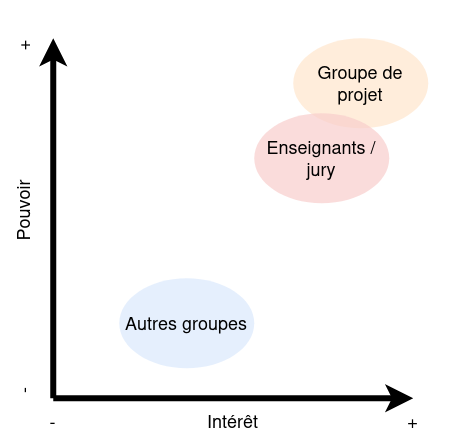
\includegraphics[width = 0.45\textwidth]{IMG/parties_prenantes.png}
\end{center}

\textbf{\underline{Plan d'action} :}
\begin{itemize}
    \item Groupe de projet : 
    \begin{itemize}
        \item Communiquer de façon régulière et transparente au sein du groupe.
        \item Organiser des réunions pour discuter des progrès réalisés, des difficultés rencontrées et des décisions à prendre.
    \end{itemize}
    \item Enseignants/jury :
    \begin{itemize}
        \item Communiquer de façon ponctuelle pour s'assurer que nous travaillons toujours dans la bonne direction.
        \item Solliciter leur aide en cas de trop grosse difficulté.
    \end{itemize}
    \item Autres groupes de projet : 
    \begin{itemize}
        \item Echanger de façon ponctuelle pour recueillir des idées, des connaissances ou des expèriences supplémentaires.
    \end{itemize}
\end{itemize}

        \subsection{Contraintes et risques}

\textbf{\underline{Contraintes} :}
\begin{itemize}
    \item Temporelle :
    \begin{itemize}
        \item Le projet doit être réalisé en 9 semaines.
    \end{itemize}
    \item Techniques :
    \begin{itemize}
        \item Langage de programmation : le langage utilisé doit être le langage "C".
    \end{itemize}
\end{itemize}
\bigskip

\textbf{\underline{Risques} :}
\begin{itemize}
    \item Techniques :
    \begin{itemize}
        \item Incompatibilités matérielles : on ne travail pas tous sous le même OS.
        \item Problèmes de performance : les outils demandés peuvent demander des traitements lourds, nos machines pourraient être dépassées.
    \end{itemize}
    \item Gestion de projet : 
    \begin{itemize}
        \item Gestion du temps et planification : on ne travail pas à temps plein sur le projet et nos autres activités peuvent nous empêcher de consacrer suffisament de temps au projet.
    \end{itemize}
    \item Liés aux données :
    \begin{itemize}
        \item Les données utilisées pour le projet peuvent être incomplètes, inexactes ou indisponibles.
    \end{itemize}
\end{itemize}
\bigskip

\textbf{\underline{Evaluation} :}
\begin{itemize}
    \item Contrainte temporelle :
    \begin{itemize}
        \item Impact : le temps disponible pour la conception, le développement et les tests est limité.
        \item Gravité : élevée, un manque de temps peut affecter la qualité globale du projet.
    \end{itemize}
    \item Contrainte technique :
    \begin{itemize}
        \item Impact : le langage "C" est maîtrisé par l'équipe, la contrainte n'a donc que peu d'impact.
        \item Gravité : Négligeable, cette contraintes peut être gérée en planifiant un temps de formation mais cela demande du temps.
    \end{itemize}
    \clearpage % --- Pour la mise en page -> à supprimer si le contenu précédent est modifié et que la mise en page change ---
    
    \item Risques techniques :
    \begin{itemize}
        \item Impact : les incompatibilités matérielles peuvent entraîner des problèmes d'intégration et de compatibilité lors de la mise en œuvre. Les problèmes de performance peuvent affecter la réactivité de l'application et la satisfaction de l'utilisateur.
        \item Gravité : Modérée, ces risques peuvent être atténués en identifiant les incompatibilités dès le début du projet et en optimisant le code pour améliorer les performances.
    \end{itemize}
    \item Risque de gestion de projet :
    \begin{itemize}
        \item Impact : Une mauvaise gestion du temps et de la planification peut entraîner des retards dans l'achèvement des tâches et la réalisation à terme des objectifs du projet.
        \item Gravité : Modérée, une bonne communication et une planification efficace peuvent minimiser les impacts de ce risque.
    \end{itemize}
    \item Risque lié aux données :
    \begin{itemize}
        \item Impact : Des difficultés pour obtenir les données peuvent allonger le temps nécessaire à l'élaboration des applications, de plus des données de mauvaise qualité peuvent affecter la précision et la validité des résultats obtenus.
        \item Gravité : Modérée, des efforts de collecte et de validation des données seront nécessaires pour minimiser l'impact de ce risque.
    \end{itemize}
\end{itemize}
\bigskip

On peut synthétiser les résultats de cette analyse dans une matrice des risques :

\begin{center}
    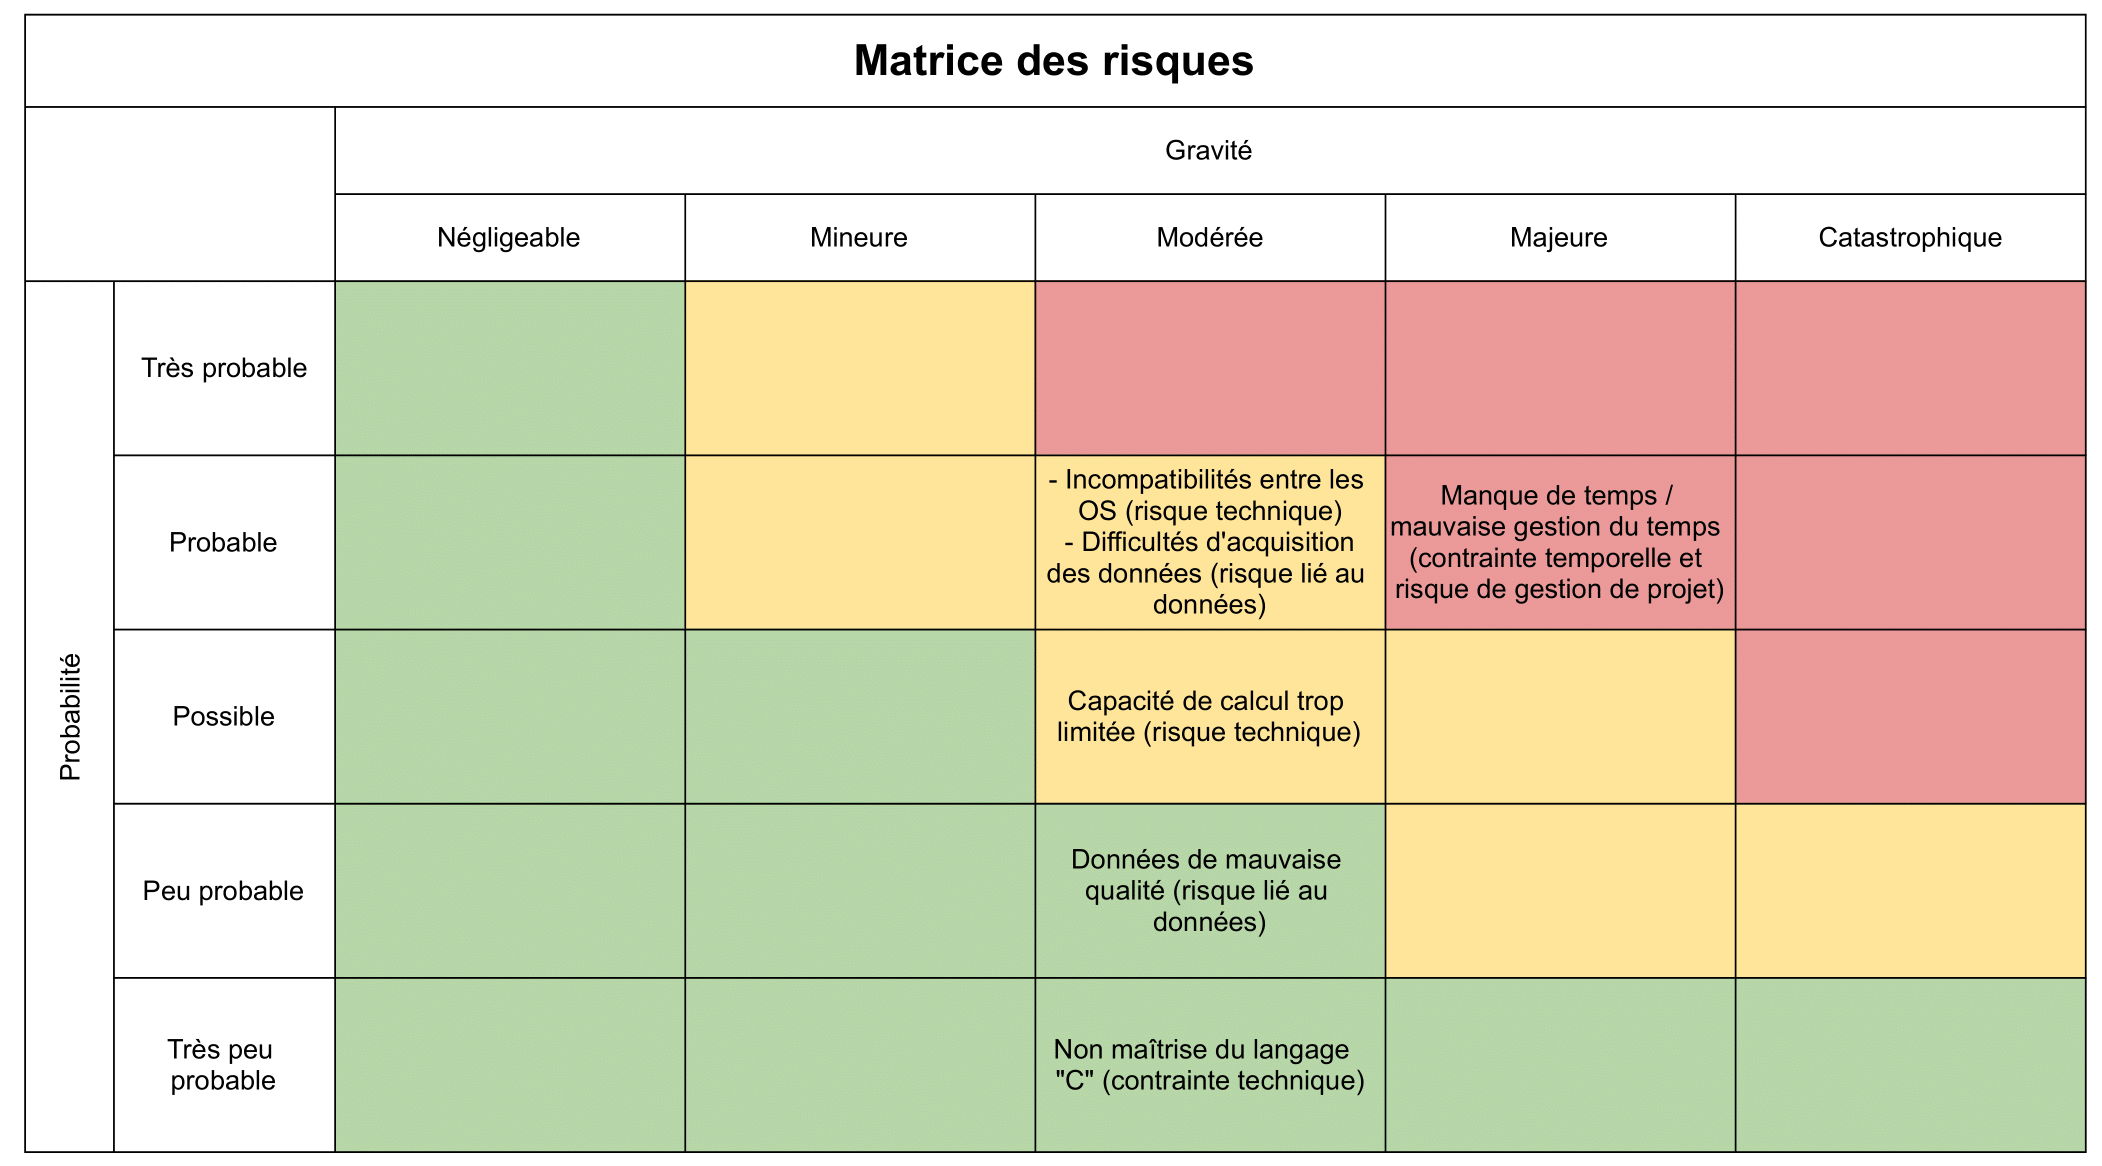
\includegraphics[width = \textwidth]{IMG/mat_risques.png}
\end{center}

\clearpage
    \section{Approche et méthodologie de gestion de projet}
        \subsection{Méthode de gestion de projet}
        \subsection{Communication et collaboration}
        \subsection{Gestion des risques}

\clearpage
    \section{Suivi et évaluation du projet}
        \subsection{Méthodes de suivi}
        \subsection{Évaluation des résultats}
        \subsection{Gestion des modifications}
        \subsection{Évaluation de la performance}
    

\chapter{Première étape}
\minitoc
\chaptermark{Première étape}
\clearpage
    \section{Analyse}
    \section{Conception et développement}
    \section{Tests et performances}


\chapter{Seconde étape}
\minitoc
\chaptermark{Seconde étape}
\clearpage
    \section{Analyse}
        \subsection{Etat de l'art}
        \subsection{Charte de projet}
    \section{Conception et développement}
    \section{Tests et performances}

\chapter{Conclusion}
\minitoc
\chaptermark{Conclusion}
\clearpage
    \section{Complétion des objectifs}
    \section{Avantages et limites du projet}
    \section{Améliorations possibles}
    \section{Clôture}

\chapter{Annexes}
\minitoc
\chaptermark{Annexes}
\clearpage            

\appendix

\end{document}